\chapter{Methodology}

\section{Proposed System Block Diagram}
\begin{figure}[h!]
    \centering
    \includegraphics[width=\textwidth]{content/images/systemBlock.png}
    \caption{Proposed system block diagram}
    \label{fig:systemBlock}
\end{figure}

The proposed system architecture in Figure 3.1 outlines the design and structure of the UTM, detailing how each component of the machine works together to simulate a Turing machine in the physical environment. The given architecture consists of several key components that interact to achieve the desired functionality of data manipulation on the memory tape. It is designed to be modular to facilitate easy understanding and construction. It integrates mechanical, electronic, and computational components that work in tandem to simulate a Universal Turing Machine's operations. In the following subsections, we present the key elements of the architecture.

\subsection{Memory Tape and Actuation System}

The memory tape serves as the primary data storage medium for the UTM. The tape is designed to be a 35mm film leader or another suitable plastic material that can be easily written to and erased. It is divided into discrete cells, each representing a binary symbol (0 or 1), with an additional blank symbol, if required, for computational purposes. Although the tape is not infinite in length, it is sufficiently long to accommodate any practical computation task. A stepper motor, controlled by an Arduino through its dedicated driver, moves the tape left or right with high precision. This ensures accurate positioning of the tape relative to the read, write, and erase heads.

The movement of the tape is regulated by a pulley system, where one full rotation of the stepper motor corresponds to the movement of one cell in either direction. This design ensures that each tape cell aligns with the heads during read, write, and erase operations, allowing for precise control over data manipulation.

\subsection{Read Head}

The read head consists of three or more CNY70 IR sensors arranged in a specific pattern to detect the reflectivity of the tape's cells. These sensors translate the reflected light from the tape into binary data, corresponding to the symbols on the tape. As the tape moves, the sensors read the state of each cell on the basis of its reflectivity, allowing the system to determine the symbol it contains.

The reflectivity data is translated into binary values as follows:

\begin{itemize}
    \item \textbf{0}: Black, White, Black
    \item \textbf{1}: White, Black, White
    \item \textbf{B}: All Black (blank)
\end{itemize}

These sensor readings are then sent to the control unit for processing, where they are interpreted and used for further computational operations.

\subsection{Write Head}

The write head is equipped with a marker controlled by two servo motors, which guide the marker along a rail. The servo motors position the marker to either write a new symbol or leave the existing symbol intact, based on the instructions provided by the control unit. This mechanism ensures that the machine can perform write operations on the tape, modifying its content as specified by the transition rules.

\subsection{Erase Head}

The erase head consists of a felt cylinder driven by a DC motor. This cylinder is used to erase the current symbol on the tape, preparing the cell for overwriting. Upon receiving an erase command from the control unit, the felt cylinder engages with the tape, clearing the symbol in the current cell.

\subsection{Control Panel}

An Arduino serves as the central control unit of the system, managing the operation of all components based on the transition rules and the initial memory configuration, which is derived from the punched card input. The control panel features input buttons that allow the user to start, stop, step through the program, load the state table, or reset the machine. An LCD display provides real-time feedback to the user, showing the current state of the Turing machine, including the content of the tape, the control state, and the operational status of the machine.

\subsection{Punched Card Reader}

The punched card reader is an essential component for reading binary data encoded in the punch cards. A microcontroller with imaging capabilities, specifically the ESP32-CAM, is employed to capture and decode the data. The ESP32-CAM takes an image of the punch card, detecting the hole patterns that represent binary data. It then processes the image, deciphers the binary patterns, and sends the decoded transition rules to the Arduino control unit. This system allows for the efficient input of computational instructions into the UTM, enabling automated program execution based on the provided punch card data.

\begin{figure}[h!]
    \centering
    \includegraphics[width=0.55\textwidth]{content/images/punchedCardReader.png}
    \caption{Working of the punched card Reader}
        \label{fig:punchedCardReader}
\end{figure}

\section{Working Principle}
\subsection{Image Processing Pipeline}

\begin{figure}[h!]
    \centering
    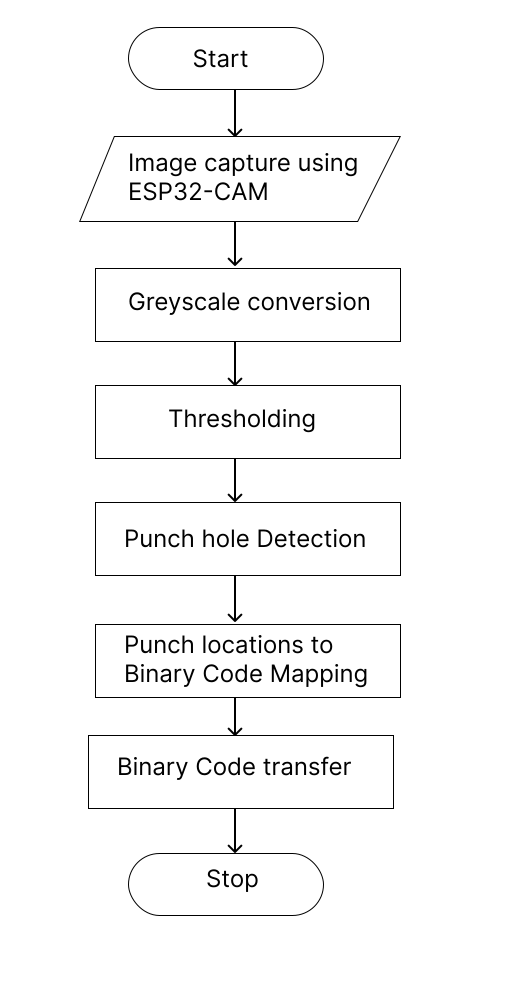
\includegraphics[width=0.5\textwidth]{content/images/imageProcessing.png}
    \caption{Proposed image processing flowchart}
        \label{fig:imageProcessingFlowchart}
\end{figure}

The flowchart in Figure~\ref{fig:imageProcessingFlowchart} illustrates the image processing steps executed by the ESP32-CAM microcontroller. The input data, provided through the punch card, is captured by the ESP32-CAM using its onboard camera. The image is processed through a series of steps outlined below. Preprocessing ensures that the captured image is suitable for decoding. This step involves several stages, including greyscaling, binarization, and edge detection.

\subsubsection{Greyscaling}
Greyscaling is the process of converting a color image, typically composed of three channels—Red (R), Green (G), and Blue (B)—into a single-channel grayscale image. Each pixel in a color image has three values, for example: \([255, 0, 0]\) for red, and \([0, 255, 0]\) for green. A grayscale image contains only one intensity value ranging from black (0) to white (255). We use the weighted method (also known as the luminosity method) to convert an RGB image to grayscale. This method accounts for the human eye’s sensitivity to different colors by applying a weight to each color channel:
\[
\text{Grayscale} = 0.299R + 0.587G + 0.114B
\]

\subsubsection{Binarization}
Binarization converts a grayscale image into a black-and-white (binary) image. This is a critical step for simplifying the image and enhancing the detection of objects or patterns. Two main methods are used for binarization: local thresholding and global thresholding.

Local thresholding calculates a threshold for each pixel based on its local neighborhood statistics. This method divides the image into smaller regions, where thresholds are calculated individually for each region based on pixel intensity variations. Local thresholding is particularly useful when dealing with images that exhibit varying lighting conditions across the image.

\begin{figure}[h!]
    \centering
    \includegraphics[width=0.8\textwidth]{content/images/localThresholding.png}
    \caption{Binarization through local thresholding}
    \label{fig:localThresholding}
\end{figure}

In Figure~\ref{fig:localThresholding}, the 16x16 grid is divided into regions, and thresholds are calculated for each region to segment elements such as grid lines and shaded areas.

Global thresholding uses the image histogram to determine a threshold. The histogram plots the pixel intensities on the x-axis and the number of pixels at each intensity on the y-axis. The threshold is typically determined as the intensity that divides the foreground from the background, and any pixel with intensity above the threshold is set to white, while pixels below it are set to black.

\begin{figure}[h!]
    \centering
    \includegraphics[width=0.8\textwidth]{content/images/globalThresholding.png}
    \caption{Binarization through global thresholding}
    \label{fig:globalThresholding}
\end{figure}

In Figure~\ref{fig:globalThresholding}, synthetic data is used to demonstrate the binarization process. The threshold divides the pixel intensities into foreground and background regions, simplifying the image for subsequent processing.

\subsubsection{Edge Detection and Region of Interest(ROI) Analysis}
Edge detection represents a critical phase in our implementation, utilizing the Sobel operator for its efficient computation and reliable results. Depending on the results during the experimentation phase, we may switch to other kernels or methods like Prewitt or CNN. The Sobel operator applies two 3x3 kernels to calculate horizontal and vertical gradients, followed by magnitude computation through the square root of their squared sums. This process effectively identifies punch card boundaries and hole edges, crucial for subsequent analysis stages.

\[
\text{Horizontal Gradient (Gx)} =
\begin{bmatrix}
-1 & 0 & 1 \\
-2 & 0 & 2 \\
-1 & 0 & 1
\end{bmatrix}
\]

\[
\text{Vertical Gradient (Gy)} =
\begin{bmatrix}
-1 & -2 & -1 \\
 0 &  0 &  0 \\
 1 &  2 &  1
\end{bmatrix}
\]

The magnitude of the gradient is computed as:
\[
\text{Magnitude} = \sqrt{Gx^2 + Gy^2}
\]

The ROI extraction follows edge detection, focusing computational resources on the relevant portions of the image. This stage implements precise boundary detection algorithms to isolate the punch card area, eliminating background noise and irrelevant features. The system then establishes a coordinate system aligned with the punch card's physical layout, creating a virtual grid that maps to potential hole locations while compensating for minor alignment deviations.

\subsubsection{Grid Mapping and Lateral Histogram Method(LAT)}

Grid mapping divides the image into a fixed grid of pre-defined rows and columns, each corresponding to a specific data point or character on the punch card. The coordinates of each grid cell are computed based on the known dimensions of the punch card, ensuring alignment with the actual punch locations.

For hole detection, we employ the LAT method which analyzes pixel intensity distributions along rows and columns. Horizontal and vertical histograms are created, showing intensity variations that indicate the presence of vertical and horizontal punch lines, respectively. Peaks in these histograms correspond to potential holes. By cross-referencing these peaks, the exact locations of the holes are determined.

\begin{table}[h!]
    \centering
    \caption{Efficiency of Lateral Histogram Method (LAT)}
    \label{tab:lat_efficiency}
    \begin{tabular}{|c|c|}
        \hline
        LAT & Efficiency Formula \\
        \hline
        LAT & \([2N^2 + (4+4r)N + 4p + (20+24r+8r^2)p^2] t_2 + 2Nt_2\) \\
        LAT' & \([2N^2 + (4+4r)N + 4p + 18p^2 + (20 + 24 + 8r^2)q^2] t_1 + 2Nt_2\) \\
        \hline
    \end{tabular}
\end{table}

Where \(N\) is the number of pixels, \(r\) is the number of edge points, \(p\) is the number of detected holes, and \(q\) is the number of true holes.

\subsubsection{Hole Classification}
Once the holes are detected, the intensity values within each cell of the grid are analyzed. Dark areas (holes) typically have lower intensity values, while light areas (non-holes) have higher intensity values. The relative intensity of each grid cell is compared to its neighbors to classify each cell as either a hole or non-hole.

\begin{example}
\[
\text{Binary Matrix:}
\begin{bmatrix}
0 & 1 & 0 \\
0 & 1 & 0 \\
1 & 0 & 1 \\
\end{bmatrix}
\]
\end{example}

In the binary matrix above, "1" represents the presence of a hole, and "0" represents no hole. This binary data is then sent to an Arduino Mega for further processing.

\section{Turing Machine Simulation - tlang}

To supplement the hardware implementation, a simulation of the Turing Machine, along with a custom language to manipulate the simulated machine, was developed to observe the machine's operations digitally \cite{tlang}. This simulation serves multiple purposes, including validating transition rules, testing various algorithms, and providing a reference for the hardware's expected behavior. tlang was implemented using C, chosen for its simplicity and efficiency, which also makes it suitable for potential porting to the hardware during the development phase.

\subsection{Design and Features}

The simulator is designed to replicate the core components and operations of a Turing Machine, featuring:
\begin{itemize}
    \item A custom language for defining the state transition table, which specifies the current state, tape symbol modification, head movement direction, and the next state for each input state-symbol pair.
    \item A memory tape represented as an extendable list, initialized with defined input data.
    \item A head pointer that moves left or right across the tape, controlled by the state transitions defined in the language.
\end{itemize}

The language comprises a minimal set of keywords: \{F, N, R, L, S, H\}, into which any arbitrary state table can be reduced. Detailed documentation of tlang's syntax and functionality is available on its GitHub page. The simulation executes step-by-step, enabling users to observe the machine's operation as it transitions through states, modifies the tape, and moves the head.

\subsection{Application and Insights}

Before the hardware implementation, the transition rules were extensively tested using the simulator. This helped identify logical errors and edge cases that could arise during execution. By simulating various scenarios, the simulator ensured the correctness of the rules and validated the feasibility of algorithms intended for the hardware. These tests provided valuable insights into the inner workings of a Turing Machine and informed design decisions for the hardware implementation.

\subsection{Visualization}

The simulator features a graphical interface that displays:
\begin{itemize}
    \item The current tape content, with the active cell highlighted.
    \item The current state of the Turing Machine.
    \item The head's position on the tape.
\end{itemize}

\begin{figure}[h!]
    \centering
    \includegraphics[width=1\textwidth]{content/images/tlang.png}
    \caption{Visualization of the tlang simulator in operation}
    \label{fig:emulatorScreenshot}
\end{figure}

\section{System Loop Flowchart}

\begin{figure}[h!]
    \centering
    \includegraphics[width=0.7\textwidth]{content/images/loopFlowchart.png}
    \caption{System Flowchart}
    \label{fig:flowchart}
\end{figure}

The state-driven process of the system begins with loading the state table and memory tape. These inputs are provided via punched cards and processed by the ESP32-CAM, which converts the punch locations into binary code. The resulting binary data is then transferred to the Arduino Mega, where both the state table and the data are loaded simultaneously with the memory tape.

The system enters a continuous loop where the current state is validated against the state table. If the state is valid, the Arduino Mega coordinates the necessary actions, including:

\begin{itemize}
    \item Moving the memory tape using the stepper motor.
    \item Controlling the read, write, and erase heads via servo motors.
    \item Processing sensor inputs.
\end{itemize}

The memory tape is modified according to the current state, and the system transitions to the next state as defined in the state table. If the halt state has not been reached, the system continues to process the next bit and repeats the loop. 

If an invalid state is encountered at any point, the process halts and displays an error message. The loop terminates only when the halt state is successfully reached, signaling the completion of the operation.

\section{Instrumentation Specification}
\subsection{Hardware Requirements}

The following hardware components are required for the project:

\begin{itemize}
    \item \textbf{Arduino Mega} (1 unit): A microcontroller board with 256KB Flash and 8KB SRAM, used for controlling project components.
    \item \textbf{ESP32 Cam} (1 unit): A 2MP camera with Wi-Fi, Bluetooth, 3.3V, and MicroSD functionality (27.5x40mm), used for image capture and processing.
    \item \textbf{Nema 17 Stepper Motor} (1 unit): A motor with 2A current and 1.8° step angle, used for precise, repeatable rotational movement.
    \item \textbf{9g Servos} (3 units): Servos with 4.8-6V, 2.5 kg.cm torque, 0.1s/60° speed, and 9g weight, used for precise angular movement and control.
    \item \textbf{Matrix Boards} (1 unit): A fiberglass board with a 2.54 mm grid and copper pads, used for prototyping and circuit connections.
    \item \textbf{White 35mm Film Leader or Lamination Sheet} (1 unit): A flexible and durable material with 35mm width that can be easily written to and erased using a marker, used as the memory.
    \item \textbf{Soldering Iron and Wire} (1 unit): A 60W soldering iron and soldering wire, used for assembling electronic components onto the matrix board.
    \item \textbf{Display and Buttons} (1 LCD and 3 push buttons): Used for user interface and input control.
    \item \textbf{3D Printed Structural Components} (multiple units): Custom-designed 3D printed parts for the physical framework.
    \item \textbf{7805 5V Regulator} (2 units): Provides a 5V output (1A max) to regulate voltage for project components.
    \item \textbf{AMS 1117 3.3V Regulator} (1 unit): Provides a 3.3V output (1A max) to regulate voltage for project components.
    \item \textbf{12V Adapter} (1 unit): A 12V DC output adapter to provide power supply to the project components.
    \item \textbf{CNY-70 IR Sensor} (1 unit): An infrared emitter and detector (5mm gap), used to output different values based on the reflectance of the surface in front of it.
    \item \textbf{Capacitors and Resistors}: 
    2 \(\times\) 10~\(\mu\text{F}\) capacitors and 
    3 \(\times\) (220~\(\Omega\), 1~k\(\Omega\)) resistors: 
    Capacitors used for the 7805 voltage regulator and resistors with CNY70 sensors as current limiter and voltage divider.
    
\end{itemize}

\subsection{Software Requirements}

\subsubsection{Arduino IDE}
An integrated development environment (IDE) for writing and uploading code to Arduino boards. It is available on Windows, macOS, and Linux platforms, and supports programming in C/C++ along with a wide range of libraries.
\subsubsection{Onshape}
A cloud-based 3D CAD software for designing and modeling electronic and mechanical parts. Onshape is platform-independent (works through browsers on Windows, macOS, and Linux). It supports parametric modeling, assemblies, and real-time collaboration. Files can be exported in common formats like STL, STEP, and IGES.
\subsubsection{EasyEDA}
An online electronic design automation (EDA) tool for circuit design, simulation, and PCB layout. EasyEDA is web-based and provides schematic capture, PCB design, and simulation tools. It supports exporting files in Gerber, PDF, and more. EasyEDA integrates with JLCPCB for PCB fabrication.
